\paragraph{V4 - Rust}

Die V4 Variante wurde ebenfalls in Rust entwickelt, aber von Grund auf neu aufgebaut. Die Architektur wurde komplett überarbeitet und stark vereinfacht. Die \Gls{statemachine} wurde verworfen und die ganze Applikation basiert auf dem Datenbank \Gls{listener}. Der Listener wurde mithilfe Funktionalität der \texttt{firestore\_rs} Softwarebilbiothek Implementiert.

\subparagraph{Projektstruktur}

Das Projekt wurde mit \texttt{cargo new} erstellt, deshalb ist die Projektstruktur wie folgt:

\dirtree{%
  .1 tower\_controller\_v4.
  .2 src.
  .3 bin.
  .3 entities.
}

\begin{itemize}
  \item \textbf{\texttt{tower\_controller\_v4}} Root Verzeichnis des Projekts, hier befinden sich alle    Konfigurationsdateien (Cargo.toml, Cargo.lock, .gitignore, etc\ldots{}).
  \item \textbf{\texttt{src}} Hier befinden sich alle Quellcode Dateien.
  \item \textbf{\texttt{bin}} Hier befinden sich alle Quellcode Dateien, die Ausgeführt werden können.
  \item \textbf{\texttt{entities}} Hier befinden sich die Serialisierbaren Datenstrukturen (Entities), die den Dokumenten in der Datenbank entsprechen.
\end{itemize}

\subparagraph{Programmablauf}
\begin{enumerate}
  \item Der Turm Controller wird mittels der \texttt{main} Funktion gestartet.
  \item Umgebungsvariablen werden geladen.
  \item Datenbank Interface wird erstellt (\texttt{TowerDatabase::new}).
  \item Turm Datenstruktur wird erstellt und mit den Daten aus der Datenbank initialisiert (\texttt{Tower::new}).
  \item Assignment Scheduler wird erstellt (\texttt{AssignmentScheduler::new}).
  \item Der Scheduler wird gestartet (\texttt{AssignmentScheduler::start}) und der main \Gls{thread} wird in einen \Gls{sleep} Modus versetzt.
  \item Das Programm wartet nun auf Änderungen in der Datenbank.
\end{enumerate}

\begin{figure}[ht]
  \centering
  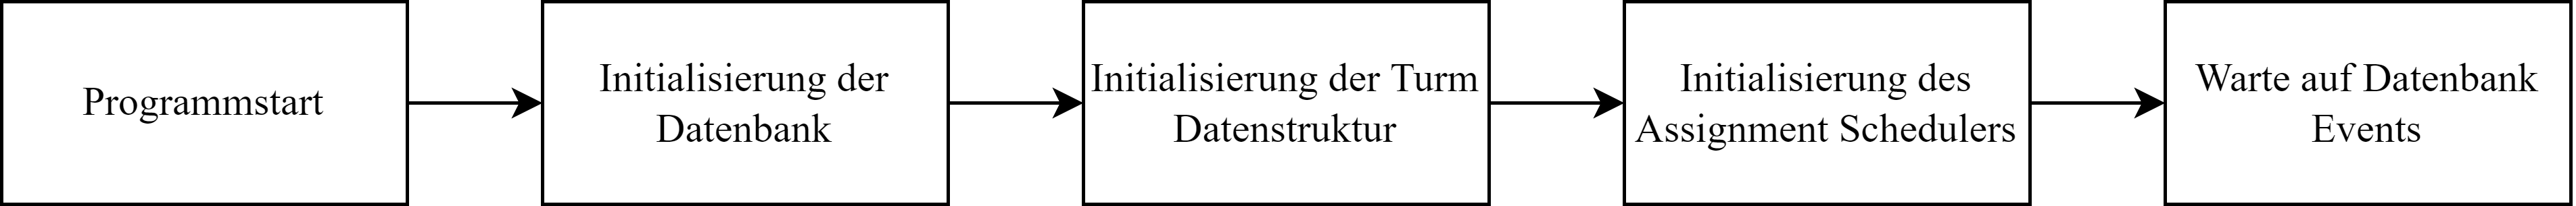
\includegraphics[width=1\textwidth]{images/tower_controller_v4_init.png}
  \caption{Intialisierung des Turm Controllers}
  \label{fig:tower_controller_v4_init}
\end{figure}

\subparagraph{{TowerDatabase}}

\texttt{TowerDatabase} kümmert sich um die Kommunikation mit der Datenbank. Es ist ein \Gls{wrapper} für die Datenbankverbindung der \texttt{firestore\_rs} Softwarebilbiothek. Es soll die interaktion mit der Datenbank vereinfachen und die möglichkeit von Fehlern minimieren.

Felder
\begin{minted}{rust}
struct TowerDatabase {
    db: FirestoreDb,
    tower_id: String,
    project_id: String,
}
\end{minted}

Methoden:
\begin{itemize}
  \item \textbf{\texttt{new}}: Erstellt eine neue Instanz von \texttt{TowerDatabase}.
  \item \textbf{\texttt{has\_subscription}}: Prüft ob ein nutzer eine Abonnement hat.
  \item \textbf{\texttt{set\_error}}: Setzt einen Fehlerstatus eines Assignments.
  \item \textbf{\texttt{set\_confirm}}: Setzt einen Bestätigungsstatus eines Assignments.
  \item \textbf{\texttt{set\_slot}}: Setzt einen Slot eines Assignments.
  \item \textbf{\texttt{create\_listener}}: Erstellt einen Listener, welcher auf Änderungen in der \texttt{jobs} Collection wartet.
  \item \textbf{\texttt{get\_tower}}: Lädt die Daten des Turms aus der Datenbank (Wichtigt für die Initialisierung des Turms).
  \item \textbf{\texttt{create\_boxes}}: Erstellt fehlende Boxen in der Datenbank anhand des Layout Felds.
  \item \textbf{\texttt{new\_rental}}: Erstellt einen neuen Mietvorgang in der Datenbank (users > rentals).
  \item \textbf{\texttt{finish\_rental}}: Beendet einen Mietvorgang in der Datenbank.
\end{itemize}


\subparagraph{Tower}

\subparagraph{AssignmentScheduler}
\begin{minted}{rust}
pub struct AssignmentScheduler {
    db: Arc<TowerDatabase>,
    tower: Arc<Mutex<Tower>>,
    listener: FirestoreListener<FirestoreDb, HashMapTokenStorage>,
}
\end{minted}


\subparagraph{TowerDisplay}
